\chapter{Problem analysis and requirements}
\label{ch:problem-analysis}

This chapter investigates the different use cases associated with cinema management and discusses potential pitfalls in the design of a generic solution. To gain a comprehensive understanding of the problem space, detailed use cases are analyzed and requirements are derived therefrom. A list of requirements is presented, which will serve as a basis for the conceptual design in the following chapter.

\section{Use cases}\label{sec:use-cases}

\todo{use-case diagram + detailed description}

An application use case diagram was created with the incoming task, which visually represents both the essential points of communication between the user and the website, as well as the configuration and use of the cinema owner and can be understood by all parties involved. The visual representation of the situation is intended to ensure that communication between all parties runs smoothly and requirements can be derived from it.

\begin{figure}[H]
    \centering
    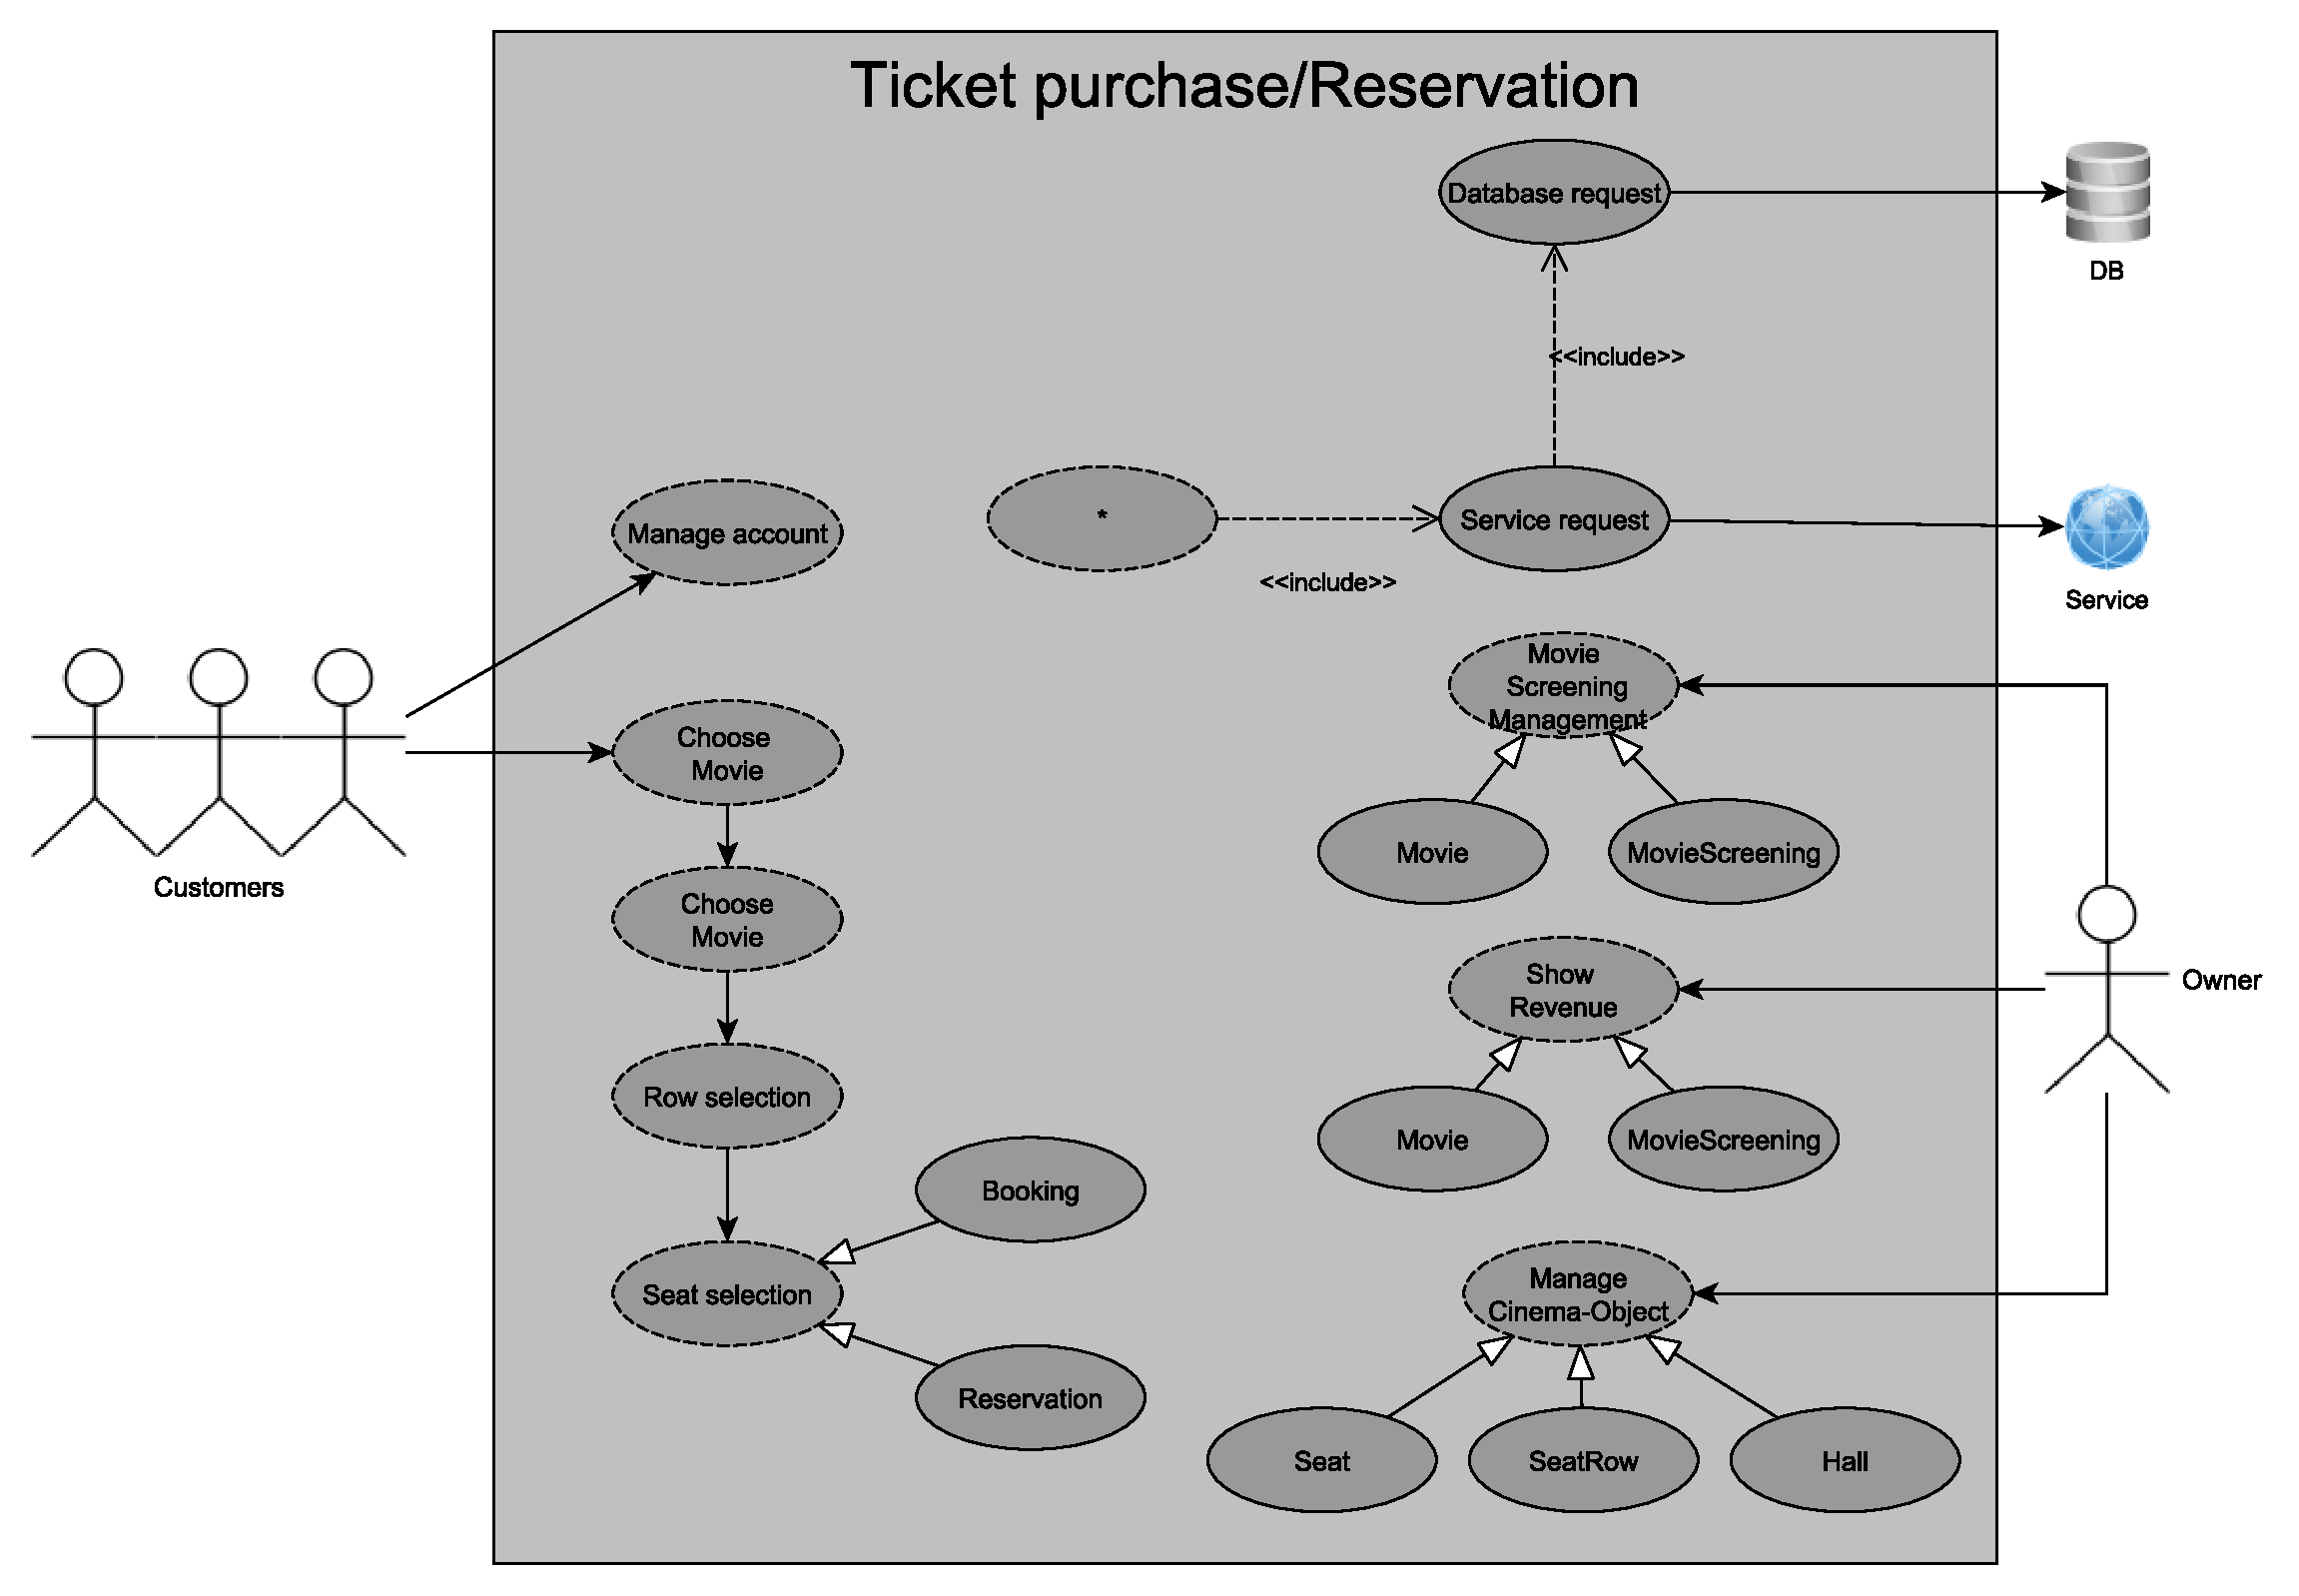
\includegraphics[width=\textwidth]{images/iis-use.case.pdf}
    \caption{Use-case diagram of reservation/ticket purchase}
    \label{fig:use-cases}
\end{figure}

The use-case diagram in Figure \ref{fig:use-cases} describes, on the one hand, the interaction of the cinema owner in the context of ticket sales/reservations, through which the owner can make various configurations to their cinema. The owner can also view their revenue. As the \enquote{Movie} and \enquote{Movie Screening} activities inherit from the \enquote{Show revenue} activity, the owner can view the total revenue of a movie or just a single screening. Furthermore, the owner can manage an entire screening (movie screening, etc.), and individual screenings can be managed because \enquote{Movie} and \enquote{Movie Screening} inherit from \enquote{Movie Screening Management}. Lastly, the owner can individually configure seats, rows, and theaters because they inherit from "Cinema Object Management".

On the other hand, the use-case diagram describes how customers can make a reservation or booking. Customers have the option to manage their created account or choose a movie. If customers choose to watch a movie, they can select their movie. After selecting their movie, they can choose which screening (different movie screenings) they want to watch the movie at. After successfully selecting the screening, the user now has the choice of which row and seat they want to sit in. When selecting a seat, the user can decide whether to book the seat immediately or reserve it first and then book it later. Upon closer inspection of the diagram, it becomes apparent that there are activities with dashed borders. All activities with dashed borders point to the activity with the name \enquote{*}, which also has a dashed border. This is for clarity and means that each of these dashed border activities involves a service request and database query.

The diagram only gives a superficial insight into the functioning of the provision of ticket sales/reservations and does not show any specific details. For this reason, the following section analyzes and defines exactly what is needed to implement the electronic sale of tickets.

\pagebreak

\section{Requirements}
\label{sec:requirements}

The investigation of the challenges elucidated in the use cases and the constraints associated therewith have led to the establishment of the following prerequisites for the proposed \gls{g:cms} solution. These requirements will serve as a basis for the conceptual design in the following chapter.

\todo{this is by no means complete :P}

\renewcommand{\arraystretch}{1.25}
\begin{table}[H]
    \centering
    \caption{Summary of requirements for \gls{g:cms}.}
    \label{tab:requirements}
    \begin{tabular}{l|p{0.75\textwidth}}
        \toprule
        Requirement & Description \\ \midrule
        \requirementdefshort\label{req:use-cases}  & \gls{g:cms} must cover the use-cases discussed in \cref{sec:use-cases}. \\ \hline
        \requirementdefshort\label{req:model-requirements}  & \gls{g:cms} must comply with all model-specific requirements specified in \cref{apx:ch:extended-analysis}. \\ \hline
        \requirementdefshort\label{req:client-server} & \gls{g:cms} must utilize the client-server architecture, allowing multiple concurrent clients to access its services. \\ \hline
        \requirementdefshort\label{req:database} & A database engine must be used to persist cinema data. \\ \hline
        \requirementdefshort\label{req:server} & The \gls{g:cms} server must be written in as a Java application complying with the principles of model driven development. \\ \hline
        \requirementdefshort\label{req:mps} & \gls{a:mps} by JetBrains must be used to generate the Java source code for data access layer and the SQL DDL required for the database schema \cite[1]{IIS2-ass}. \\ \hline
        \requirementdefshort\label{req:mysql} & \gls{g:cms} data must be persisted in a MySQL database. \\ \hline
        \requirementdefshort\label{req:isolation} & Database access must be performed in a thread-safe and isolated manner. \\ \hline
        \requirementdefshort\label{req:api} & The server must provide a \gls{a:rest}ful \gls{a:json} \gls{a:api} for the client application to communicate with, as established in \todo{use-case here}. \\ \hline
        \requirementdefshort\label{req:client-access} & The client application must be able to connect to the server via a \gls{a:rest}ful \gls{a:json} \gls{a:api}. \\ \hline
        \requirementdefshort\label{req:client-cli} & A \gls{a:cli} must be provided for user interaction within the client application. \\ \hline
        \requirementdefshort\label{req:client-portability} & The client application must be capable of being published as a self-contained executable, guaranteeing portability without reliance on any additional runtime environment for installation. \\ 
        \bottomrule
    \end{tabular}
\end{table}
\renewcommand{\arraystretch}{1}